\section{Tower design}
As mentioned in our section on requirements, our projectile launcher has some firm requirements. It needs to be able to detect, aim and fire at a moving target. 
From a design perspective we need two distinct properties namely, horizontal and vertical rotation. There are of course many different ways of achieving both horizontal and vertical rotation, but in our case the simplest thing would be to have one servo motor handle vertical rotation and another servo motor to handle horizontal rotation. 

Now we need to figure out how many degrees do we need to rotate. If we want full 360 degree rotation then everything needs to be mounted on a platform, including the NXT and possibly the Kinect camera, both of which are relatively heavy. With this approach the weight of the structure might become an issue, as we intend to use a single servo motor to handle the horizontal rotation. The big question is whether the servo is strong enough to rotate the platform fast enough to hit a moving target. We decided to test whether this approach could meet our requirements.

 We started out with a base construction illustrated in figure~\ref{base}, and we were planning on mounting the firing mechanism (hereafter referred to as the turret) on top of the base. On close inspection of the figure~\ref{base} there is a cross axle in the center that handles all of the rotation.

\begin{figure}[hptb]
  \centering
    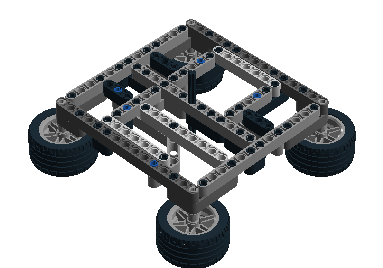
\includegraphics[width=0.5\textwidth]{img/base.png}
  \caption{Initial base construction}
  \label{base}
\end{figure}

Figure~\ref{first_model} depicts the initial design. The construction was quite simply too top heavy thus making it difficult to achieve a precise and reliable rotation. If we were going to use this construction, we needed a large and completely smooth surface between the base and the turret. We tried, but were unable to find an acceptable solution. The main problem was that a single servo was responsible for rotating the everything except the base, and the servo even had to handle its own weight. The rotation was achieved through gears and leavers rotated by a single servo, which also put a lot of strain on the cross axle that the structure was being rotated around.

\begin{figure}[hptb]
  \centering
    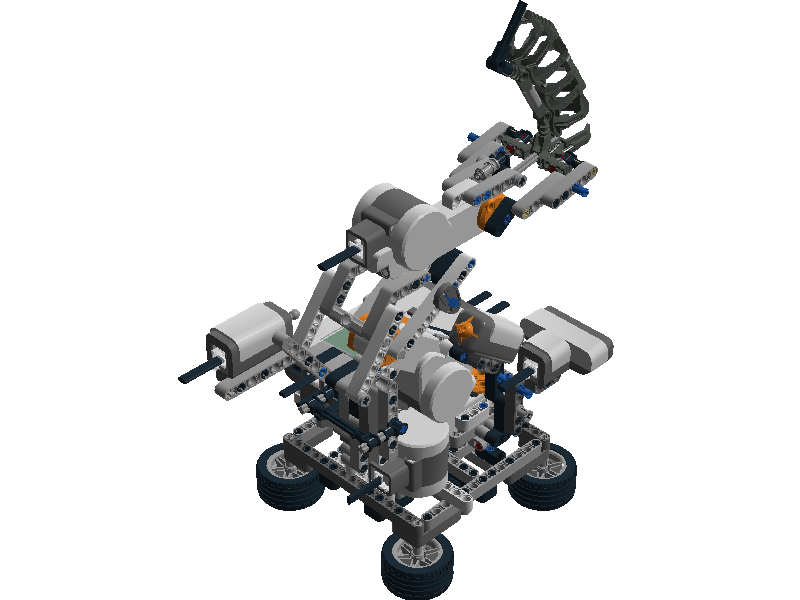
\includegraphics[width=1.0\textwidth]{img/Step114.png}
  \caption{Initial model for the projectile launcher}
  \label{first_model}
\end{figure}

Figure~\ref{final_model} shows the final design of the projectile launcher. In our final design we focused on minimizing the weight on the rotating turret, so we then opted for a design where a minimal set of components handled the vertical rotation and firing and the horizontal rotation was refactored in such a way that we could remove it from the turret and the rotation was restricted to a fixed set of degrees. This decision was based on the hardware analysis where we discovered that the Kinect only can detect objects within a 60 degree angle. The turret itself had to refactored to only contain the parts necessary for the construction to meet it's requirements, this meant that the NXT and the Kinect did not have to be placed on the turret, but rather behind and in front of the turret. We could place the servo that handled horizontal rotation on a structure that stood next to the turret. And lastly we needed some way of configuring the starting position of the turret, in order to be absolutely sure that the turret was facing in the same direction on every initialization. So we placed a pressure sensor next to the turret and mounted a beam onto the turret that would hit the sensor at a certain angle. It should also be noted that the actual firing mechanism, depicted in figure~\ref{competition_cannon} we are using is a LEGO piece called a "Competition cannon", but this piece is not included in LEGO Digital Designer, which we used to make the model. 

\begin{figure}[hptb]
  \centering
    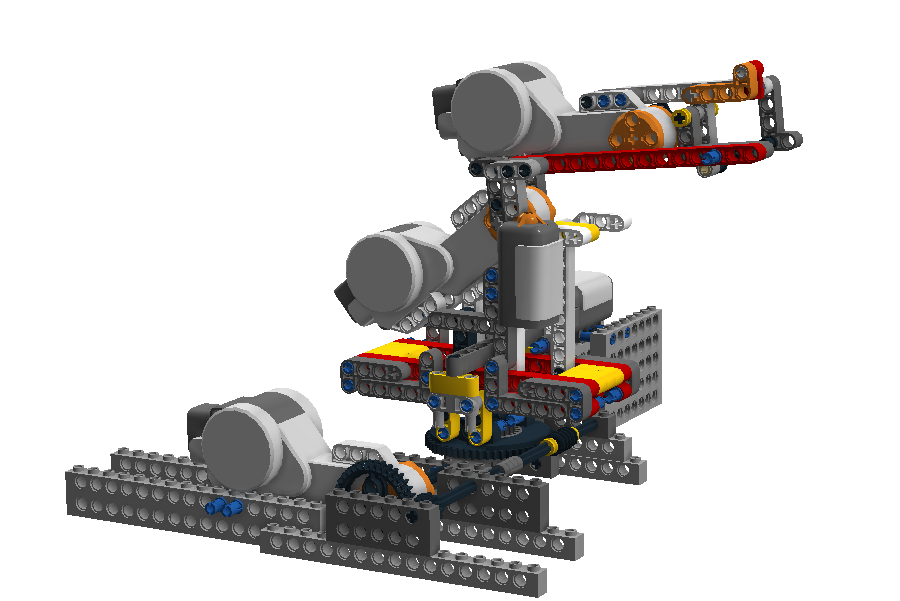
\includegraphics[width=1.0\textwidth]{img/design_turret4.png}
  \caption{Final model of the projectile launcher.}
  \label{final_model}
\end{figure}

\begin{figure}[hptb]
  \centering
    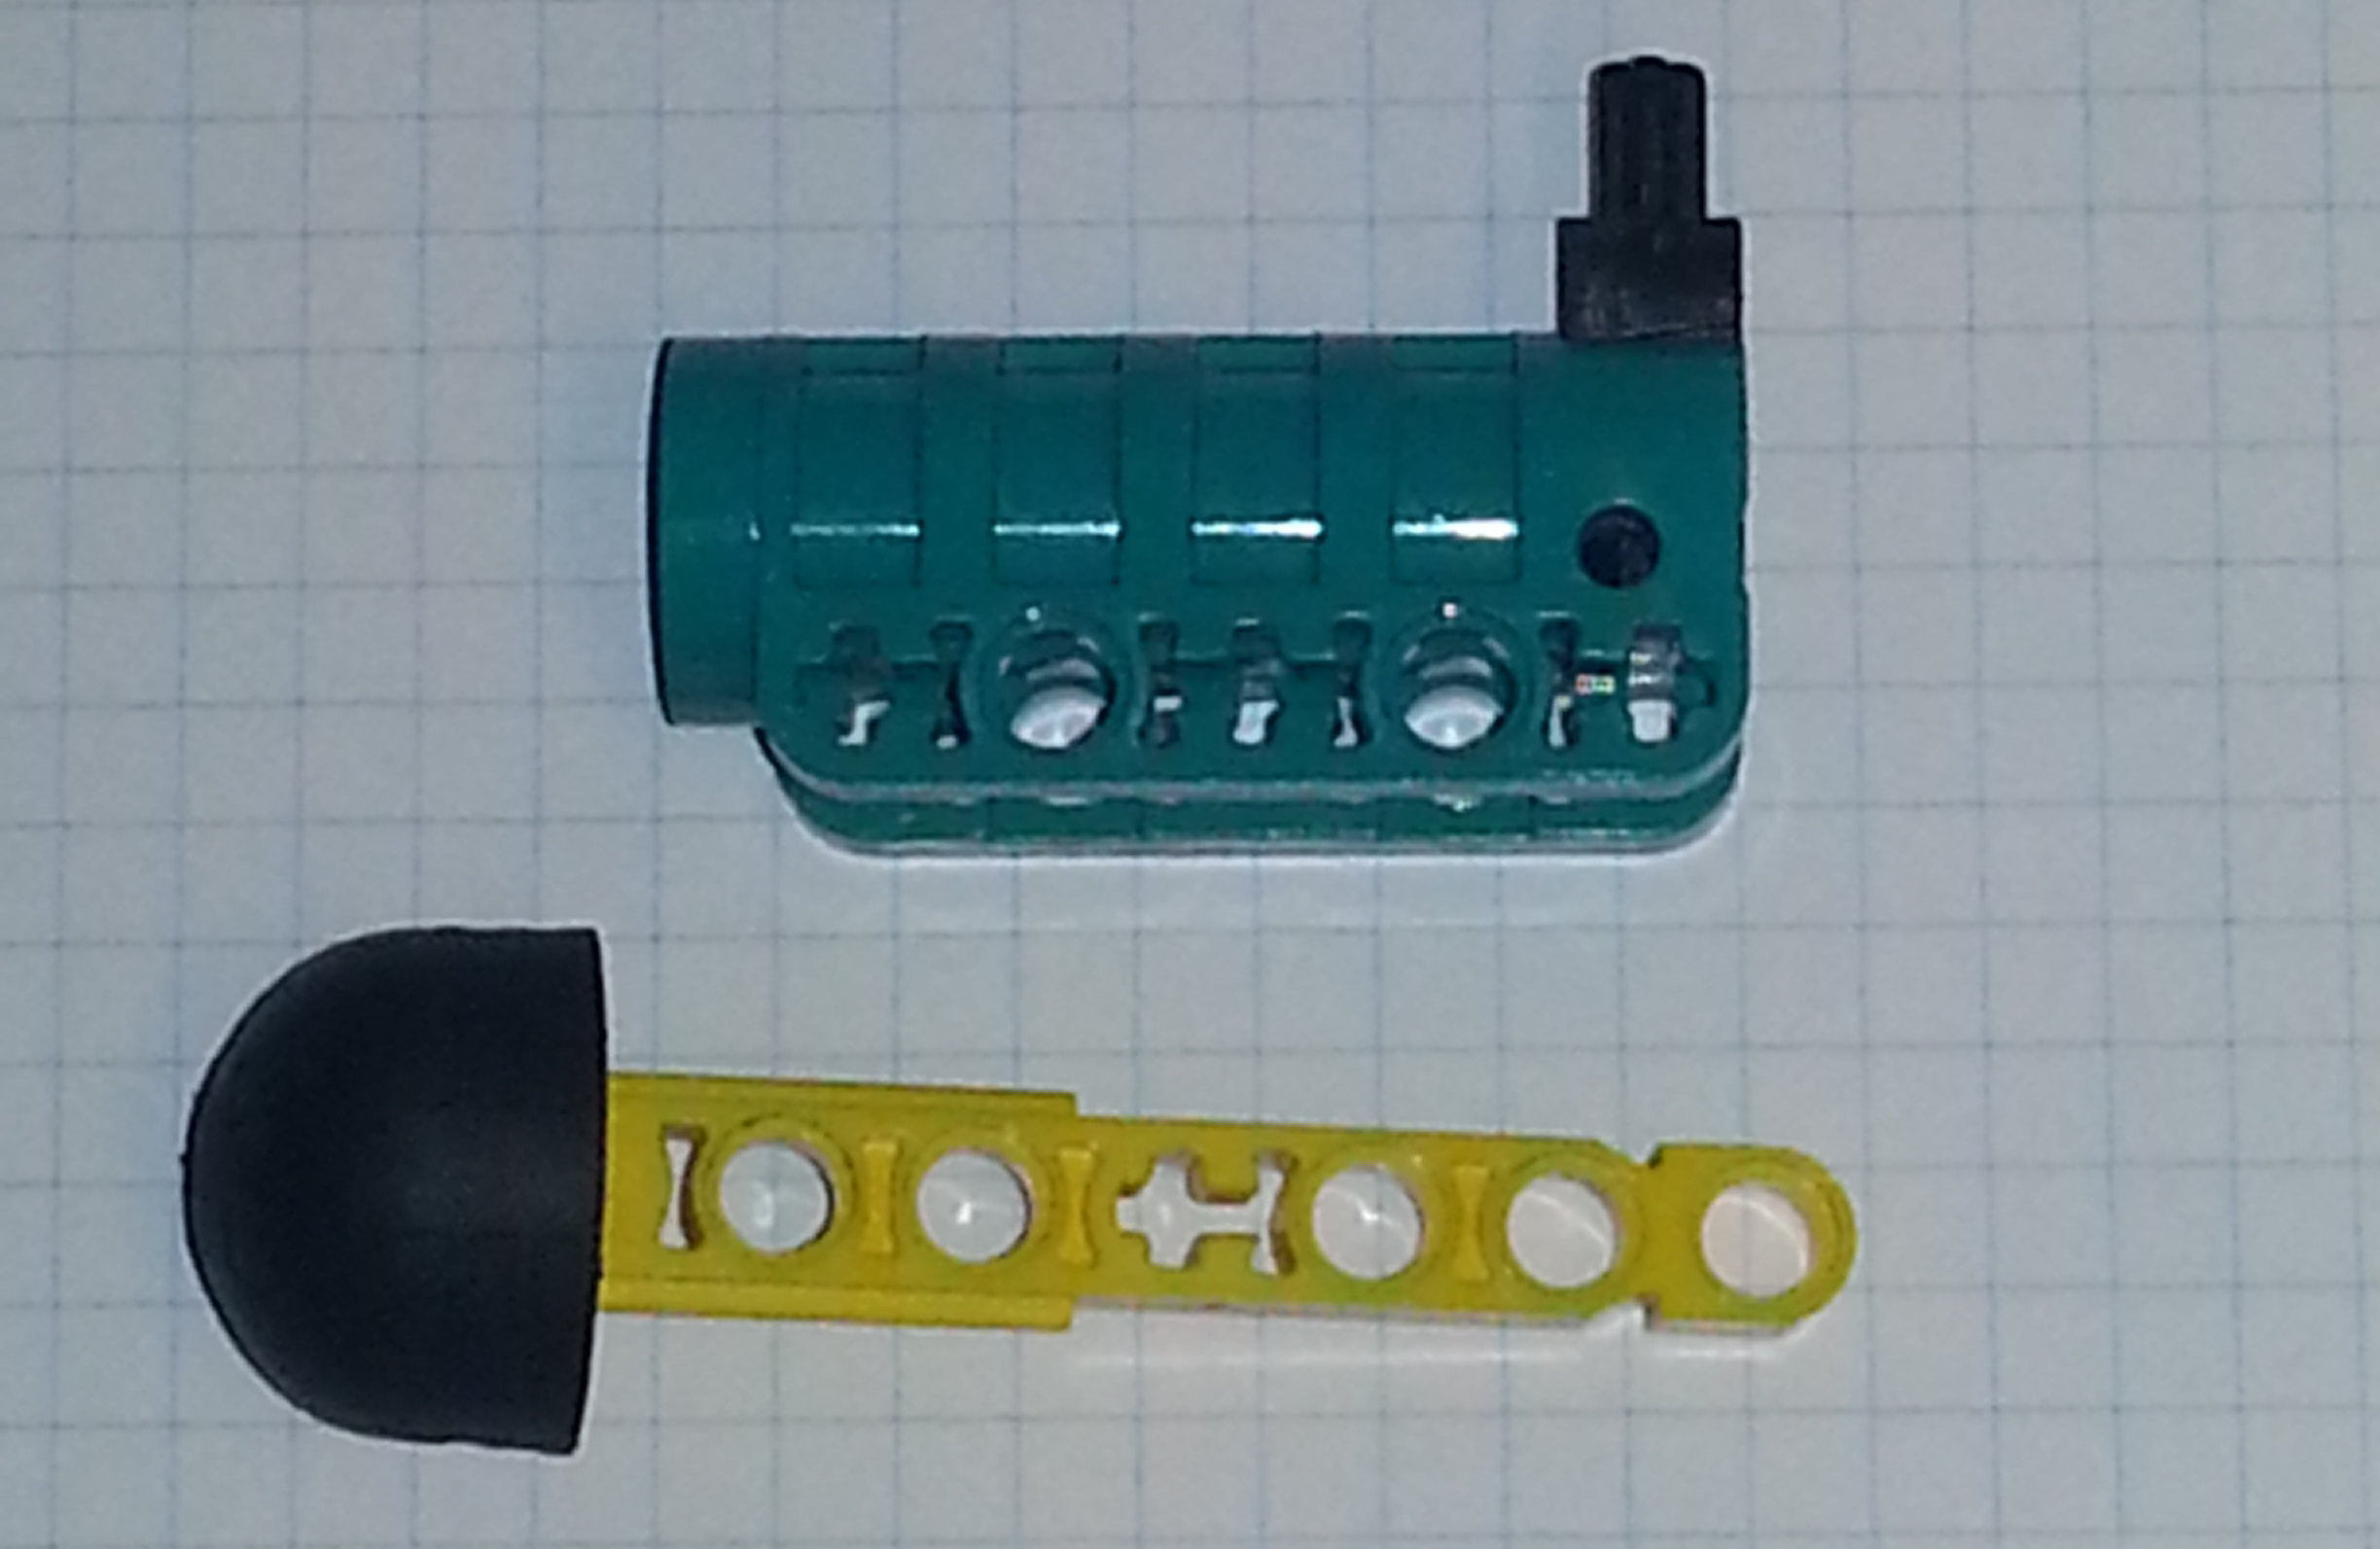
\includegraphics[width=0.5\textwidth]{img/competition_cannon.png}
  \caption{Our projectile firing mechanism}
  \label{competition_cannon}
\end{figure}

\subsection{Placing the Kinect} % (fold)
\label{sub:placing_the_kinect}
There are several options with regards to the placement of the Kinect in relation to the Projectile Launcher. The ideal solution would probably be to place the Kinect right onto a rotating the turret with the possibility of 360 degree rotation, this would enable the Projectile Launcher to hit targets all around it. However this proved inefficient with regards to weight distribution and stability.

Another approach would be to place the Kinect behind or next to the turret, with the turret within the Kinect's field of vision. This would enable the Kinect to calculate the target's position and speed in relation to the turret. The problem is that the turret would also obstruct the Kinect's field of vision, resulting in irregularities and might even lead to false calculations.

A third approach, and the one we implemented, is to place the Kinect right in front of the turret, directly under the actual cannon. In this case we only have to calculate the height difference between the Kinect and the cannon. The Kinect can only see a limited amount of degrees on the horizontal axis, and we have configured the turret to be able to rotate accordingly. Thus fulfilling the requirements.
%subsection placing_the_kinect (end)